\documentclass{article}
\usepackage{amsmath}
\usepackage{graphicx}
\title{IVP Analytic vs. Numerical Solution}

\begin{document}

\maketitle

\section{Problem}

Compare the analytic and numerical solution of $\eta$ of the following shallow water problem:

\[
\begin{aligned}
\eta = e^{-(x-3.5)^2} \\
u = 0 \\
h = x \\
m = \infty  \\
\end{aligned}
\]

In other words, a Gaussian initial wave with no initial velocity, and a plane-inclined shape ($y^\infty$). This reduces to a 1-1 SWE. We can reproduce this with a different slope and initial conditions easily.

\section{Setup}

Statistical comparison was done on an equally spaced grid of 1000 points in time on [0,3] and at 1000 points in x on [-2.5, 6.5]


\subsection{Numerical}

I set Deny's Catalina 1 "runwave.m" with the initial conditions. The following displays eta in the $(x,t)$ plane

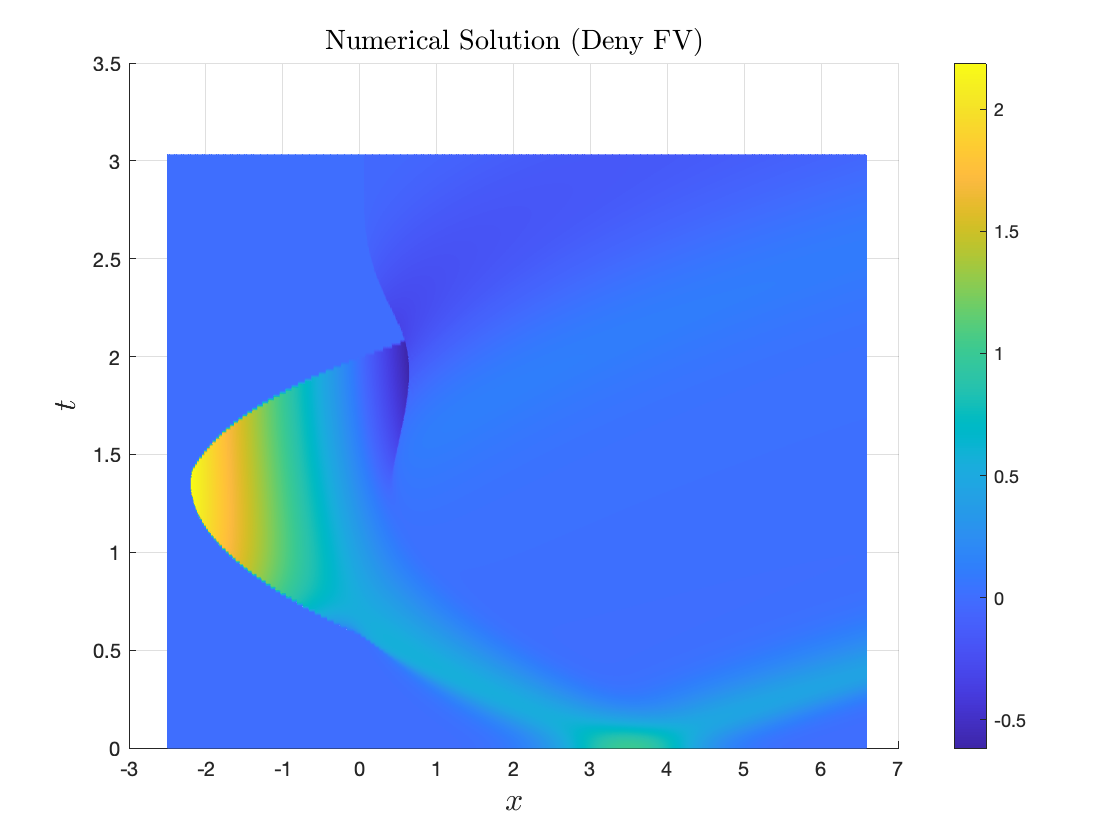
\includegraphics[width=\linewidth]{num.png} 


\subsection{Anaylytic}

Chebfun was used to calculate the Hankel transform solution to the CG transform on a grid in $(s,\lambda)$ then CG transform to $(x,t)$

\noindent The following figure shows the a grid in $(s,\lambda)$ transformed to $(x,t)$

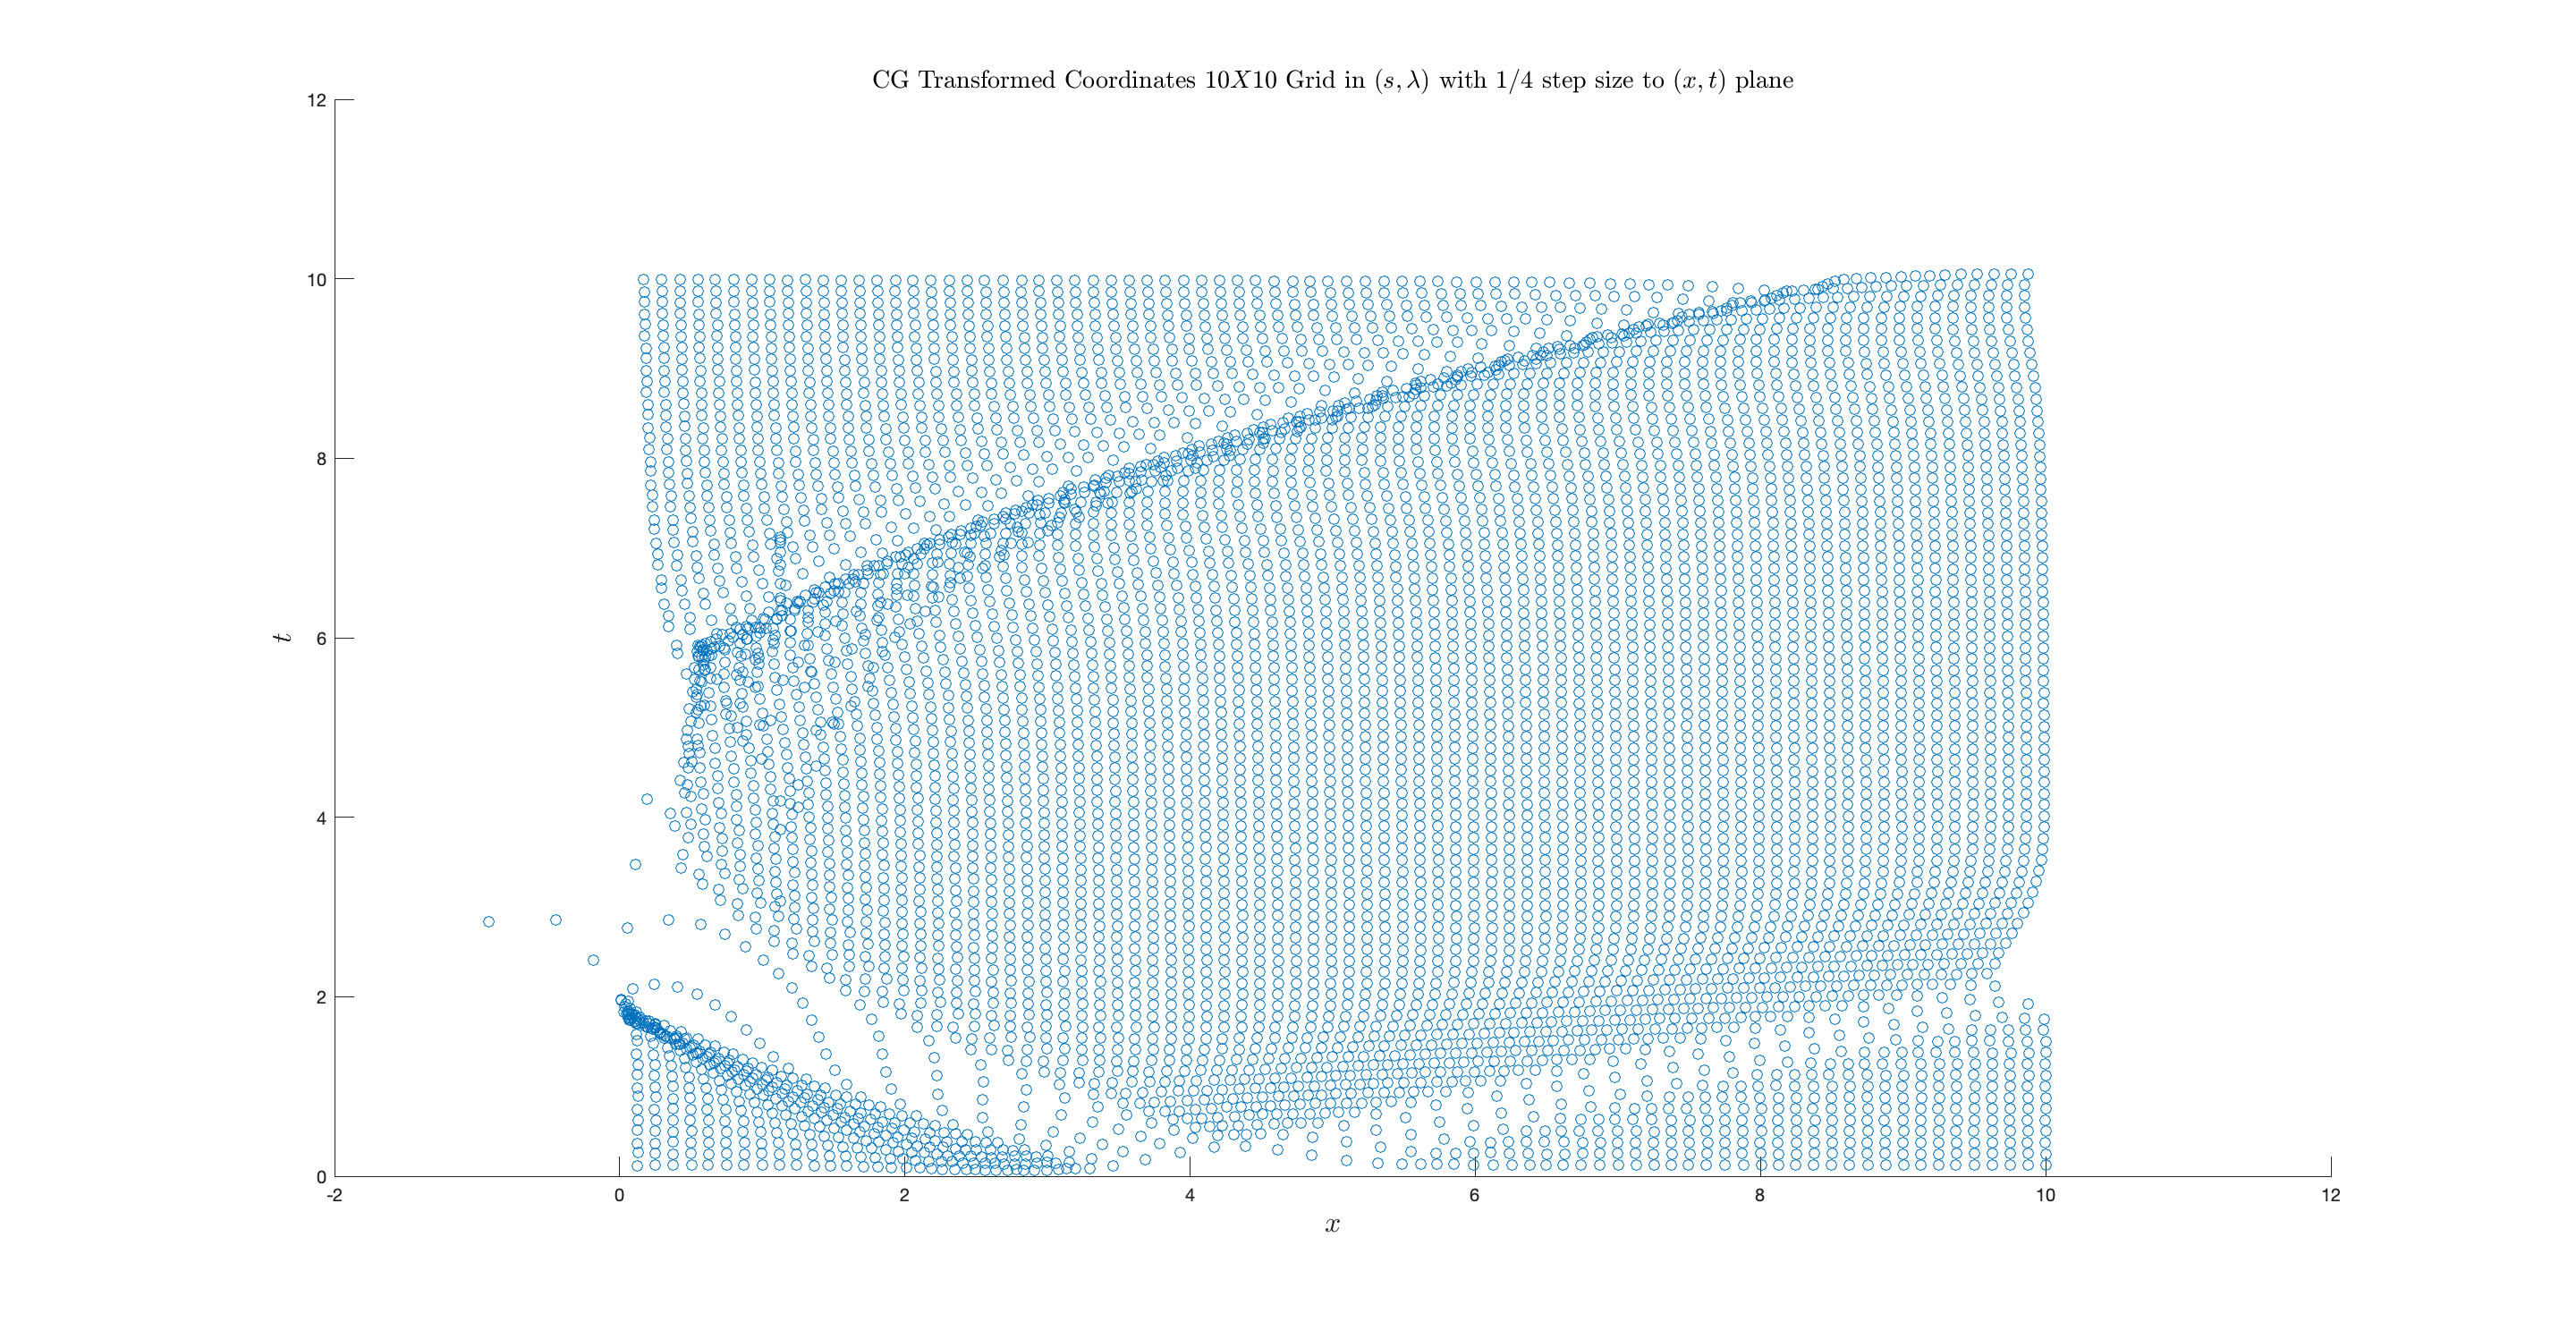
\includegraphics[width=\linewidth]{images/scatter.png} 

\noindent Note the distinct non-linear nature caused by the $-u^2$ of $\eta$

\noindent The analytical solution of $\eta$ was computed using formulas in Nicolsky (2018)

\[
\begin{aligned}
\psi (s, \lambda ) = \int_{0}^\infty (a(k)cos(\beta k \lambda)+b(k)*sin(\beta k \lambda) )dk \\
\phi (s, \lambda ) =  \\
\end{aligned}
\]

where

\[
\begin{aligned}
a(k) = e^{-(x-3.5)^2} \\
b(k) =  \\
\end{aligned}
\]

\[
\begin{aligned}
a(k) = e^{-(x-3.5)^2} \\
b(k) =  \\
\end{aligned}
\]

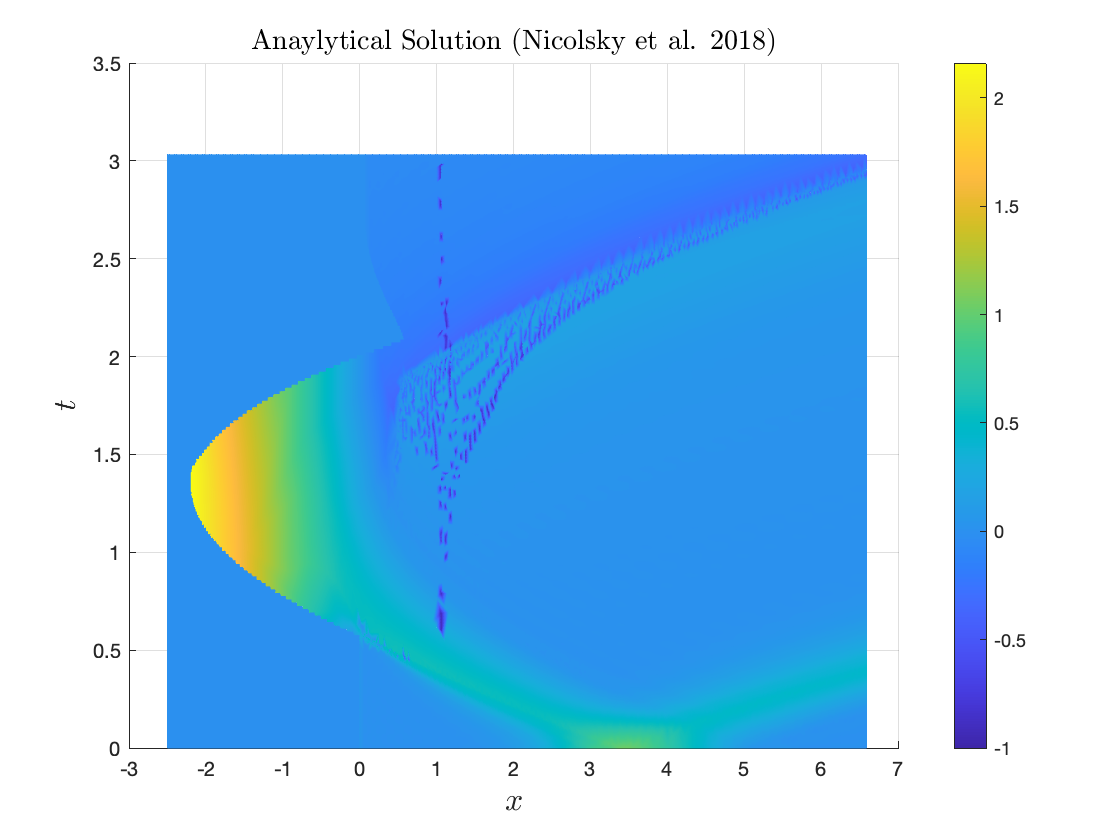
\includegraphics[width=\linewidth]{ana.png}

\section{Statistical Analysis}

This is the difference between the two ie. numerical - anaytical

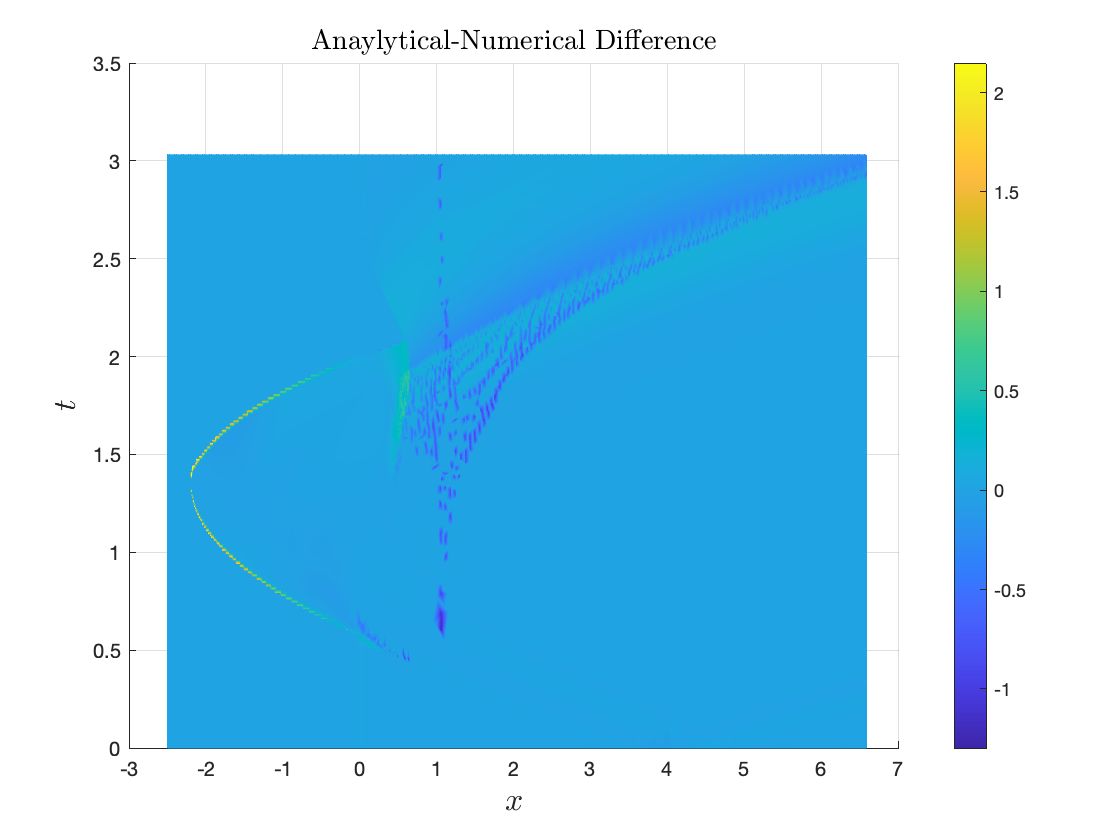
\includegraphics[width=\linewidth]{diff.png}

\noindent The following is the L2 norm at each value of t. The difference increases in a sporadic fashion at the beginning and end of run-up. The primary explaination for this is problems with the computation of the analytic solution.


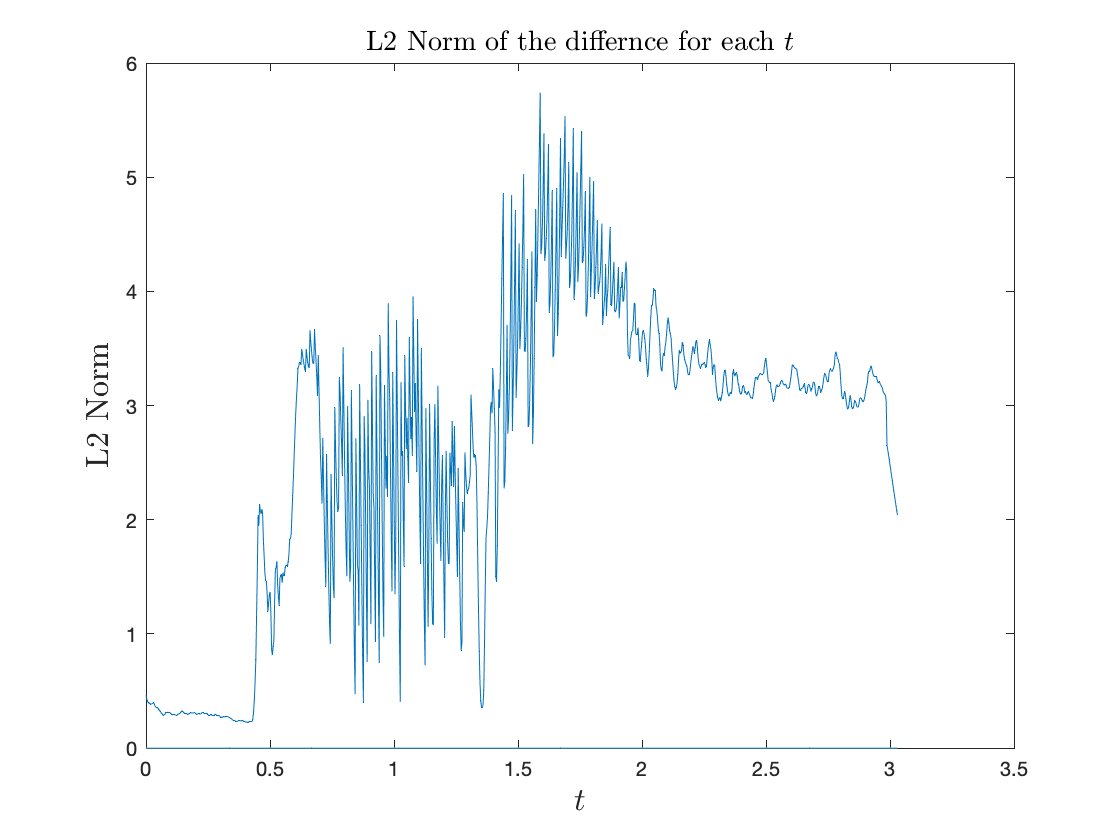
\includegraphics[width=\linewidth]{l2.png}

\section{Further Problems}

1. Analytic solution stability.

\noindent2. Comparison of the speed wasn't completed.

\noindent3. Different initial conditions.

\noindent4. NOAA anaytic solution.

\end{document}
